\chapter{Computation of the fifth action}    \label{chapter-6}



\section{Problems in trying to compute the spin sector action integral while flowing under $\Eff$}


Under the $\Eff$ flow, we have the following
EOMs.
\begin{equation}
\begin{aligned}
&\frac{d \vec{R}}{d \lambda}=\vec{S}_{\mathrm{eff}} \times \vec{R} , \\
&\frac{d \vec{P}}{d \lambda}=\vec{S}_{\mathrm{eff}} \times \vec{P} ,  \\
& \frac{d \vec{S}_{a}}{d \lambda} =\sigma_{a}\left(\vec{L} \times \vec{S}_{a}\right),
\end{aligned}
\end{equation}
which further imply that
\begin{equation}
\begin{aligned}
\frac{d \vec{L}}{d \lambda} &=\vec{S}_{\mathrm{eff}} \times \vec{L}.
\end{aligned}
\end{equation}


We now try to compute the contribution to the action integral.
We get
\begin{equation}    \label{J5_1}
\begin{aligned}
&2 \pi \mathcal{J} =2 \pi\left(\mathcal{J}^{\mathrm{orb}}+\mathcal{J}^{\mathrm{spin}}\right) \\
&=\int_{\lambda_{i}}^{\lambda_{f}}\left(P_{i}  {d R^{i}}
+  S_1^z {d \phi_1^z}
+  S_2^z {d \phi_2^z}
\right)     \\
&=\int_{\lambda_{i}}^{\lambda_{f}}\left(P_{i} \frac{d R^{i}}{d \lambda}
+  S_1^z \frac{d \phi_1^z}{d \lambda}
+  S_2^z \frac{d \phi_2^z}{d \lambda}
\right) d \lambda
\end{aligned}
\end{equation}
Let's focus only on the orbital part.
\begin{equation}    \label{J5_orb_B}
2 \pi \mathcal{J}^{\text {orb }}=\int_{\lambda_{i}}^{\lambda_{f}} \vec{P} \cdot\left(\vec{S}_{\mathrm{eff}} \times \vec{R}\right) d \lambda=\int_{\lambda_{i}}^{\lambda_{f}}\left(S_{\mathrm{eff}} \cdot L\right) d \lambda=\left(S_{\mathrm{eff}} \cdot L\right) \Delta \lambda
\end{equation}
where we have used $S_{\mathrm{eff}} \cdot L$ to represent
$\Eff$. It could be pulled out of the integral because it is a constant 
during the $\Eff$ flow, i.e. $d{\Eff}/d \lambda =  \pb{\Eff, \Eff} = 0$.



So, the orbital sector of the integral was simple. But we have no idea how
to do the spin sector integral. Note that the simplicity of the orbital sector 
integral is owed to $\vv{L}$ being written as a cross product
$\vv{L} = \vec{R} \times \vec{P}$. The same is not true for the spins, which makes
it impossible to do the spin sector integral in Eq.~\eqref{J5_1}.





\section{Computing the spin sector  contribution to the action integral using the extended phase space}



\subsection{Introducing the fictitious variables}

The main reason the spin sector contribution to the action integral
while flowing under $\Eff$ is that spins can't be written 
a cross product of some positions and some momenta, the way $\vv{L}$
can be. This motivates us to introduce unmeasurable, fictitious variables
$\vv{R_{a}}$ and $\vv{P_{a}}$ with $a = 1, 2$ such that
\begin{equation}
\vec{S}_{a} \equiv \vec{R}_{a} \times \vec{P}_{a}  . 
\end{equation}
With these fictitious variables, the spins are no longer the 
independent, fundamental coordinates but now they rather depend on
the fictitious variables. We now introduce some simple 
terminology. 
The totality of $\vec{R}, \vec{P}, \vec{S}_1$ and $\vec{S}_2$
forms the standard phase space (SPS).
The totality of $\vec{R}, \vec{P}, \vec{R}_{1/2}$ and $\vec{P}_{1/2}$
forms the extended phase space (EPS). 
The vectors $\vec{R}_{1/2}$ and $\vec{P}_{1/2}$ form the sub-spin space.




Many things need to be put on a firm footing with the 
introduction of these new fictitious variables. We do so one by one.
\begin{itemize}
\item \textbf{Hamiltonian:} The Hamiltonian will now be seen
as a function of the EPS coordinates, rather than the SPS ones.
\item \textbf{Poisson brackets:} PBs need to be defined, for the EOMs are written
in their terms. We propose
\begin{equation}
\left\{R_{i}, P_{j}\right\} =\delta_{ij}, \quad\left\{R_{ai}, P_{b j}\right\}=\delta_{a b} \delta_{ji}      \label{EPS_PBs}
\end{equation}
\item \textbf{EOM:} The EOMs are still given by the same familiar equation
\begin{equation}
\frac{d f}{d t}=\{f, H\}
\end{equation}
\item \textbf{Equivalency of the SPS and the EPS pictures in terms of EOMs:}
The only reason we can introduce the EPS picture is that the EPS
picture is completely equivalent to the SPS one, i.e. the EOMs for all
real (non-fictitious) variables are the same in the two pictures.

Why do we say that? This is because the EPS PBs imply the SPS PBs, i.e.
Eqs.\eqref{EPS_PBs} $\implies$  Eqs.~\ref{C1-canonical PB}.
\item \textbf{Equivalency of the SPS and the EPS pictures in terms of integrability:}
The system is integrable even in the EPS picture. To show that
we need to come up with $n = 2n/2 = 18/2 = 9$ commuting constants in the EPS picture.
Five of them are the SPS commuting constants (see Eq.~\eqref{C1-CCs})
but considered functions of the EPS coordinates and not the SPS coordinates.
The next four are $S^2_{1/2}$ and $\vec{R}_{1/2} \cdot \vec{P}_{1/2}$.
\item \textbf{Sanity check 1:} All observables should depend only on non-fictitious variables alone. This is indeed the case. All five actions we derive depend only 
on $\vec{R}, \vec{P}, \vec{S}_1$ and $\vec{S}_2$ and the two masses; 
any dependence on the fictitious variables is through $\vec{S}_1$ and $\vec{S}_2$.
Although actions are not observables, frequencies $\omega_i = \pd H / \pd \mc{J}_i$
are; and they are a functions of non-fictitious variables only.
\item \textbf{Sanity check 2:} We have checked numerically that the fifth action
(computed with the help of fictitious variables), when seen as a function of 
the SPS coordinates only, generates a flow which forms a closed loop after 
flowing by $2 \pi$ within numerical errors.
\item \textbf{An EPS action is also an SPS action:} If we succeed in computing
an EPS action which is a function of ($\vec{R}, \vec{P}, \vec{S}_1$ and $\vec{S}_2$),
then this should also serve as an SPS action. How? Our EPS action flow 
must make a loop in the EPS. The same action when seen as  a function of the SPS
coordinates must also make a loop in the SPS. This is because the PBs are the 
same in the SPS and the EPS and flow equations are written using PBs. 
Since the flow of the EPS action (when seen as  a function of SPS coordinates)
makes a closed loop in the SPS, it can also be considered as a legitimate action in
the SPS.
\end{itemize}





\hfill \break


\begin{definition}[label=def:F]
There is small hole in the argument presented above regarding the EPS
action being also the SPS action. What if the EPS action loop 
(obtained by flowing under the fifth action by $2 \pi$)
corresponds to a loop in the SPS which goes around more than once.
We require actions to make a closed loop  \textit{just once}
when we flow under them and the above possibility is undesirable.
But this is not  a cause for worry because in Ref.~\cite{tanay2021action},
we invoke some topology arguments to rule this out.
\end{definition}

\hfill \break





\begin{tcolorbox}
The method of inventing temporary spurious variables is not that
uncommon. We use complex contour integration methods to compute integrals
which are cast in terms of reals and whose result is also real.
See Sec.~11.8 of Ref.~\cite{arfken2013mathematical}. 
In this case, the complex numbers can be thought of as temporary spurious
variables invented to solve some problem which was cast in terms of fewer
variables (reals).
\end{tcolorbox}





\subsection{Computing the spin sector of the action integral under the $\Eff$ flow}



In the EPS picture, under the $\Eff$ flow the EOMs are
\begin{equation}
\begin{aligned}
\frac{d \vec{R}}{d \lambda} &=\vec{S}_{\mathrm{eff}} \times \vec{R} ,  \\
\frac{d \vec{P}}{d \lambda} &=\vec{S}_{\mathrm{eff}} \times \vec{P} , \\
\frac{d \vec{R}_{a}}{d \lambda} &=\sigma_{a}\left(\vec{L} \times \vec{R}_{a}\right) ,\\
\frac{d \vec{P}_{a}}{d \lambda} &=\sigma_{a}\left(\vec{L} \times \vec{P}_{a}\right).
\end{aligned}
\end{equation}
The contribution to the action integral becomes
\begin{equation}
\mathcal{J}_k=\frac{1}{2 \pi} \oint_{\mathcal{C}_{k}}\left(\vec{P} \cdot d \vec{R}+\vec{P}_{1} \cdot d \vec{R}_{1}+\vec{P}_{2} \cdot d \vec{R}_{2}\right),
\end{equation}
which further entails that
\begin{align}
&2 \pi \mathcal{J}_{S_{\text {eff }} \cdot L}=2 \pi\left(\mathcal{J}^{\text {orb }}+\mathcal{J}^{\text {spin }}\right)\\
&=\int_{\lambda_{i}}^{\lambda_{f}}\left(P_{i} \frac{d R^{i}}{d \lambda}+P_{1 i} \frac{d R_{1}^{i}}{d \lambda}+P_{2 i} \frac{d R_{2}^{i}}{d \lambda}\right) d \lambda\\
&=\int_{\lambda_{i}}^{\lambda_{f}}\left(\vec{P} \cdot\left(\vec{S}_{\mathrm{eff}} \times \vec{R}\right)+\vec{P}_{1} \cdot\left(\sigma_{1} \vec{L} \times \vec{R}_{1}\right)\right.\\
&\left.+\vec{P}_{2} \cdot\left(\sigma_{2} \vec{L} \times \vec{R}_{2}\right)\right) d \lambda\\
&=2 \int_{\lambda_{i}}^{\lambda_{f}}\left(S_{\mathrm{eff}} \cdot L\right) d \lambda=2\left(S_{\mathrm{eff}} \cdot L\right) \Delta \lambda_{S_{\mathrm{eff}} \cdot L}\\
&\mathcal{J}_{S_{\mathrm{eff}} \cdot L}=\frac{\left(S_{\mathrm{eff}} \cdot L\right) \Delta \lambda_{S_{\mathrm{eff}} \cdot L}}{\pi},   \label{J5_seffdl}
\end{align}
which is just twice the contribution of 
the orbital part given in Eq.~\eqref{J5_orb_B}.



\begin{tcolorbox}
Basically, with the introduction of the fictitious variables, and expanding the 
SPS to EPS, we bring the spins at the same mathematical footing as $\vec{L}$, in that
all three of them can be written as cross products of some position with some 
momentum. This renders the otherwise insoluble spin sector contribution
to the action integral under the $\Eff$ flow rather trivial to deal with (the way
orbital sector contribution is), as if it was meant to be.
\end{tcolorbox}



\section{Computing the fifth action}


\subsection{Setting up the stage}


We will only outline the steps needed to compute the fifth action. For details,
refer to Ref.~\cite{tanay2021action}. To compute the fifth action,
a flow only under $\Eff$ is not enough; it won't make a closed loop.
In the SPS space, to close the loop, we further need to flow under
$J^2$ and $L^2$, whereas in the EPS space, we need two more flows 
($S_1^2$ and $S_2^2$ flow) on the
top of that because we have extra variables in the EPS. Because we know
how to compute the action integral  contribution corresponding
to $\Eff$ flow only in the EPS, we will try to close the loop in the EPS.
The successive flows we need are those of $\Eff, J^2, L^2, S_1^2$ and $S_2^2$.
At this point, we mention the result that under the flow by 
the last four 
constants of motion, the contribution to the action integral is 
\begin{equation}
\begin{aligned}
&\mathcal{J}_{J^{2}}=\frac{J^{2} \Delta \lambda_{J^{2}}}{\pi} , \\
&\mathcal{J}_{L^{2}}=\frac{L^{2} \Delta \lambda_{L^{2}}}{\pi}, \\
&\mathcal{J}_{S_{1}^{2}}=\frac{S_{1}^{2} \Delta \lambda_{S_{1}^{2}}}{\pi}, \\
&\mathcal{J}_{S_{2}^{2}}=\frac{S_{2}^{2} \Delta \lambda_{S_{2}^{2}}}{\pi}.
\end{aligned}
\end{equation}
These are easy to derive and can be derived in an
analogous manner as contribution corresponding to the first
constant $\Eff$ was derived in Eq.~\eqref{J5_seffdl}. Therefore the 
fifth action becomes
\begin{equation}     \label{J5_final}
\begin{aligned}
\mathcal{J}_{5}=& \frac{1}{\pi}\left\{\left(S_{\mathrm{eff}} \cdot L\right) \Delta \lambda_{S_{\mathrm{eff}} \cdot L}+J^{2} \Delta \lambda_{J^{2}}+L^{2} \Delta \lambda_{L^{2}}
+S_{1}^{2} \Delta \lambda_{S_{1}^{2}}+S_{2}^{2} \Delta \lambda_{S_{2}^{2}}\right\} .
\end{aligned}
\end{equation}
The problem of determining the fifth action thus reduces to determining 
the flow amounts needed (under various commuting constants) to close the loop.





\subsection{Determining the flow amounts}







\subsubsection{$\Eff$ flow}

Under the $\Eff$ flow the magnitudes of all the three 3D position and 
momentum vectors stay constant. So does the magnitude of all the three
angular momenta. The effect of $\Eff$ flow on the three angular momenta 
is shown in Fig.~\ref{seffdl_flow}. The triad formed by the three
angular momenta acts like a lung and it ``inhales'' and ``exhales''.
All three mutual angles between the angular momenta are periodic functions
of the flow parameter with the same period $\Delta \lambda_{\Eff}$.
See Ref.~\cite{tanay2021action}
for the derivation of these results. So, naturally we want to flow 
under $\Eff$ by exactly by a multiple of this period because if we 
did not, then there is very little hope of restoring all the coordinates
to their initial state by flowing under other constants. This
is so because other constants do not change these mutual angles
between the three angular momenta (except for the Hamiltonian).
So, we decide to flow under $\Eff$ by an amount $\Delta \lambda_{\Eff}$.




\subsubsection{$J^2$ flow}

It's shown in Ref.~\cite{tanay2021action} that by an appropriate amount
$\Delta \lambda_{J^2}$ of flow under $J^2$, we can restore all the three angular momenta to their initial states.


\subsubsection{$L^2, S_1^2, S_2^2$ flow}

Because all three angular momenta have been restored, the only
way $\vec{R}, \vec{P}, \vec{R}_{1/2}$ and $\vec{P}_{1/2}$ off from their 
initial state is by a some finite rotation in the plane perpendicular
to $\vec{L}$ (for $\vec{R}, \vec{P}$) 
and $\vec{S}_{1/2}$ (for $\vec{R}_{1/2}, \vec{P}_{1/2}$). To negate this offset,
all we need to do is to flow under $L^2, S_1^2$ and $S_2^2$ by some
appropriate amounts. This is also worked out in Ref.~\cite{tanay2021action}.
Once these amounts are determined, Eq.~\ref{J5_final}
finally yields the fifth action variable.





\begin{figure}
  \centering
  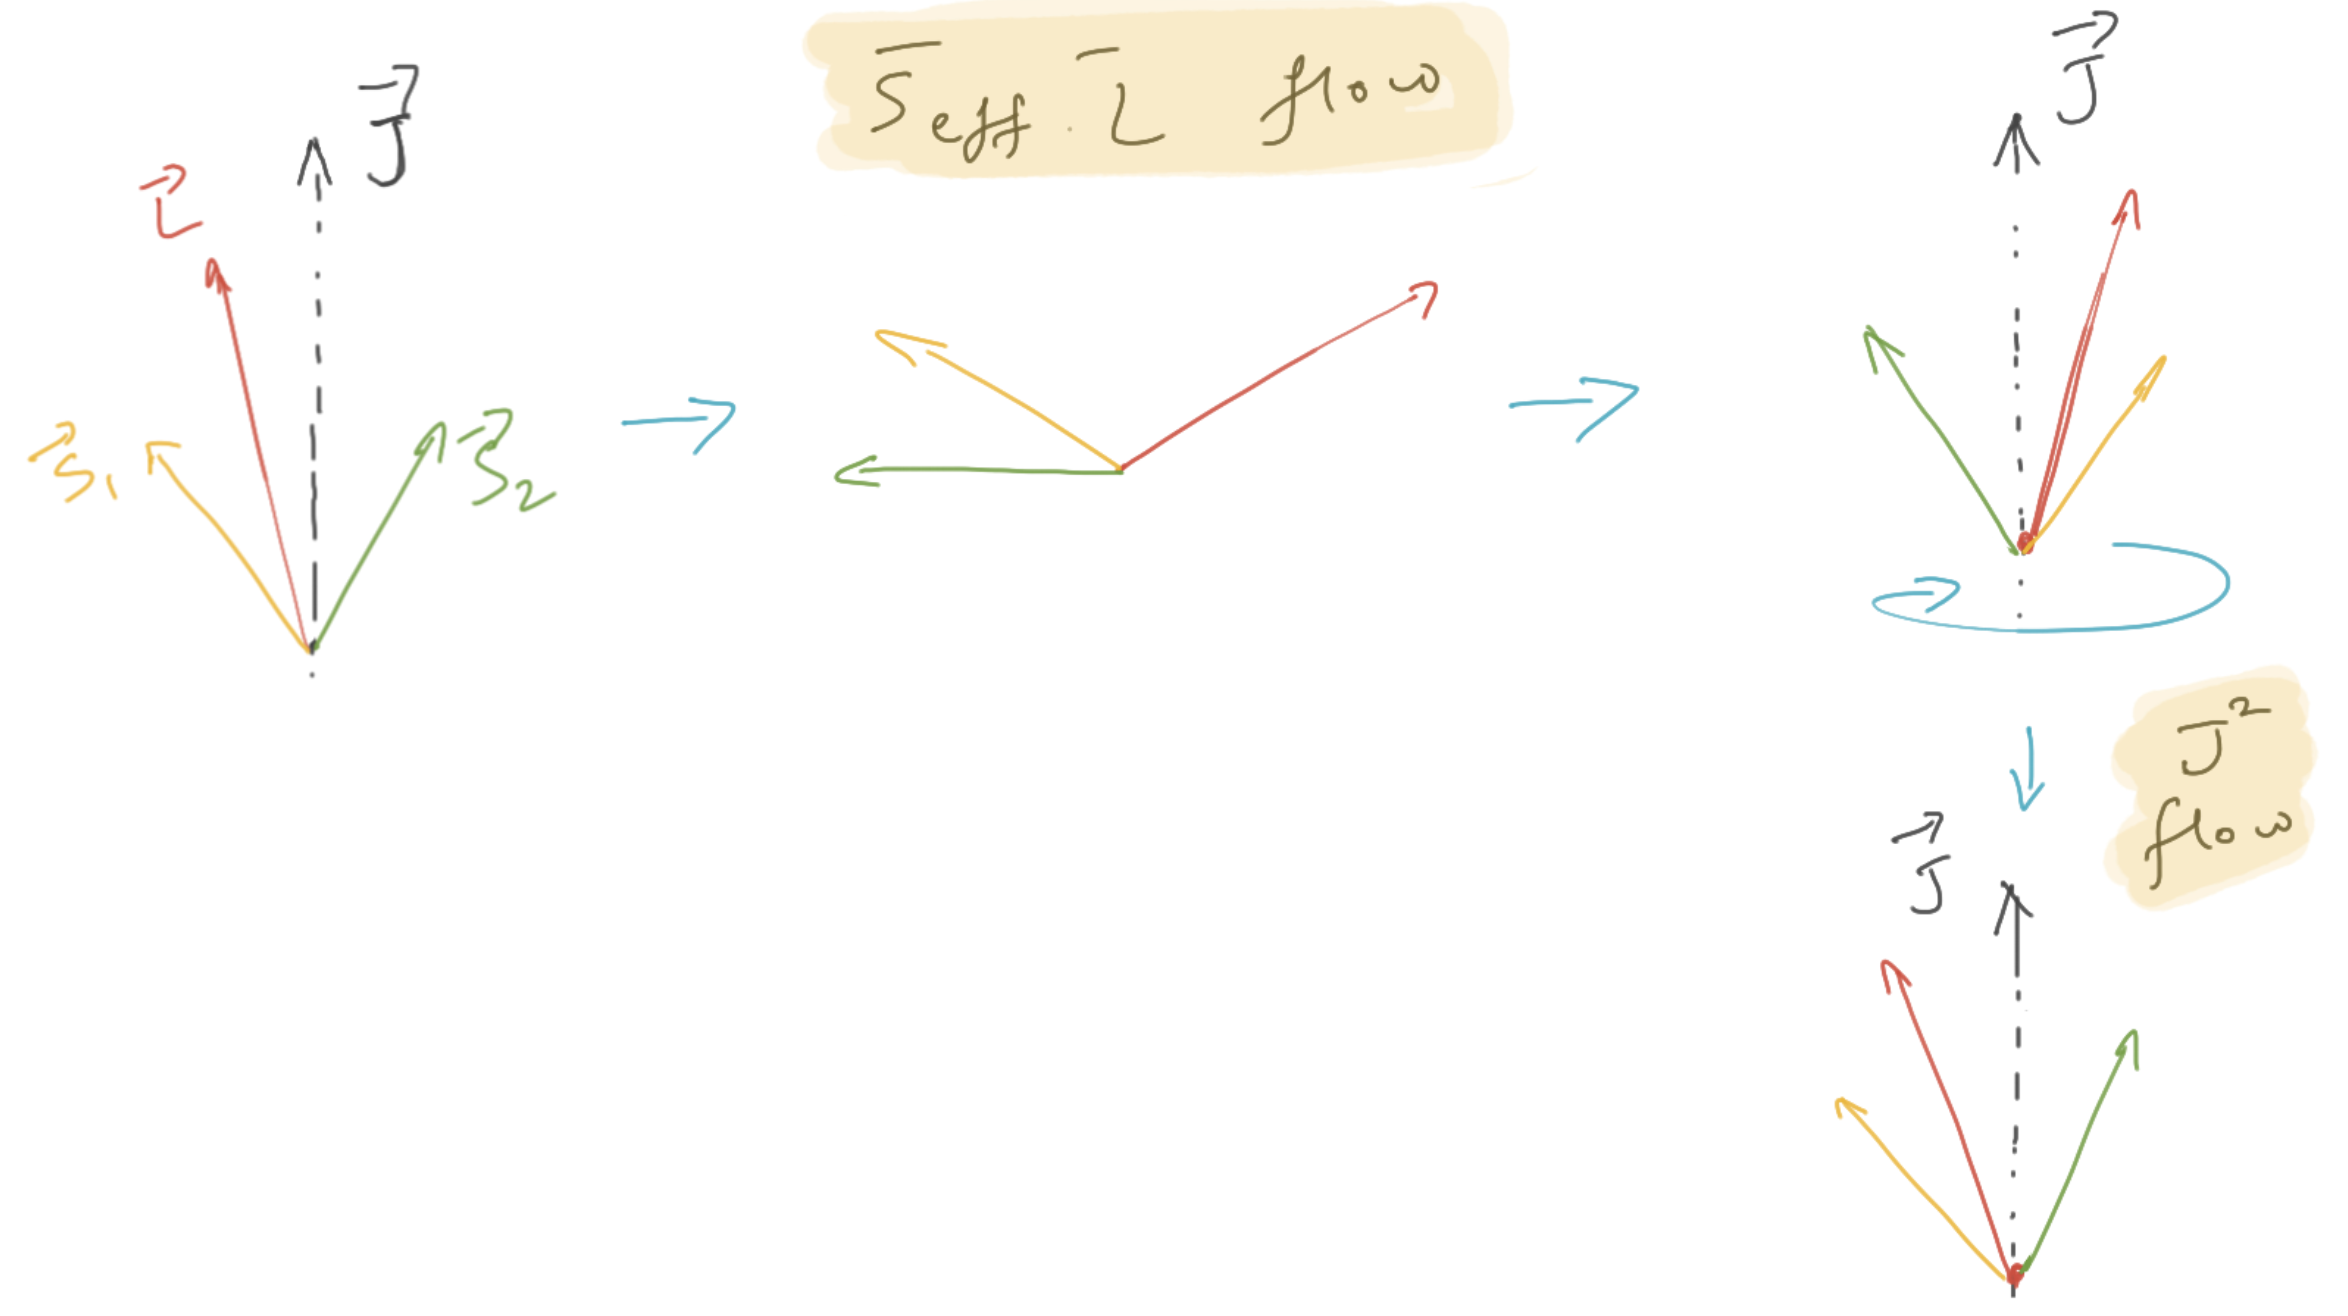
\includegraphics[width=0.8\linewidth]{seffdl_flow}
  \caption{ Behavior of the angular momenta under 
  the $\Eff$ flow.
    \vspace{-1.em}
  }
  \label{seffdl_flow}
\end{figure}
















